% $Id: template.tex 11 2007-04-03 22:25:53Z jpeltier $

\documentclass{vgtc}                          % final (conference style)
%\documentclass[review]{vgtc}                 % review
%\documentclass[widereview]{vgtc}             % wide-spaced review
%\documentclass[preprint]{vgtc}               % preprint
%\documentclass[electronic]{vgtc}             % electronic version

%% Uncomment one of the lines above depending on where your paper is
%% in the conference process. ``review'' and ``widereview'' are for review
%% submission, ``preprint'' is for pre-publication, and the final version
%% doesn't use a specific qualifier. Further, ``electronic'' includes
%% hyperreferences for more convenient online viewing.

%% Please use one of the ``review'' options in combination with the
%% assigned online id (see below) ONLY if your paper uses a double blind
%% review process. Some conferences, like IEEE Vis and InfoVis, have NOT
%% in the past.

%% Figures should be in CMYK or Grey scale format, otherwise, colour
%% shifting may occur during the printing process.

%% These few lines make a distinction between latex and pdflatex calls and they
%% bring in essential packages for graphics and font handling.
%% Note that due to the \DeclareGraphicsExtensions{} call it is no longer necessary
%% to provide the the path and extension of a graphics file:
%% \includegraphics{diamondrule} is completely sufficient.
%%
\ifpdf%                                % if we use pdflatex
  \pdfoutput=1\relax                   % create PDFs from pdfLaTeX
  \pdfcompresslevel=9                  % PDF Compression
  \pdfoptionpdfminorversion=7          % create PDF 1.7
  \ExecuteOptions{pdftex}
  \usepackage{graphicx}                % allow us to embed graphics files
  \DeclareGraphicsExtensions{.pdf,.png,.jpg,.jpeg} % for pdflatex we expect .pdf, .png, or .jpg files
\else%                                 % else we use pure latex
  \ExecuteOptions{dvips}
  \usepackage{graphicx}                % allow us to embed graphics files
  \DeclareGraphicsExtensions{.eps}     % for pure latex we expect eps files
\fi%

%% it is recomended to use ``\autoref{sec:bla}'' instead of ``Fig.~\ref{sec:bla}''
\graphicspath{{figures/}{pictures/}{images/}{./}} % where to search for the images

\newcommand{\figref}[1]{\hyperref[#1]{Figure~\ref*{#1}}}
\usepackage{xspace}
\newcommand{\ie}{{i.e.}\xspace}
\newcommand{\eg}{{e.g.,}\xspace}
\newcommand{\cf}{{c.f.}\xspace}
\newcommand{\ea}{{et~al.}\xspace}
\newcommand{\aka}{{a.k.a.}\xspace}
\newcommand{\etc}{{etc.}\xspace}

\usepackage{microtype}                 % use micro-typography (slightly more compact, better to read)
\PassOptionsToPackage{warn}{textcomp}  % to address font issues with \textrightarrow
\usepackage{textcomp}                  % use better special symbols
\usepackage{mathptmx}                  % use matching math font
\usepackage{times}                     % we use Times as the main font
\renewcommand*\ttdefault{txtt}         % a nicer typewriter font
\usepackage{cite}                      % needed to automatically sort the references
\usepackage{tabu}                      % only used for the table example
\usepackage{booktabs}                  % only used for the table example
%% We encourage the use of mathptmx for consistent usage of times font
%% throughout the proceedings. However, if you encounter conflicts
%% with other math-related packages, you may want to disable it.

%% If you are submitting a paper to a conference for review with a double
%% blind reviewing process, please replace the value ``0'' below with your
%% OnlineID. Otherwise, you may safely leave it at ``0''.
\onlineid{0}

%% declare the category of your paper, only shown in review mode
\vgtccategory{Research}

%% allow for this line if you want the electronic option to work properly
\vgtcinsertpkg

%% In preprint mode you may define your own headline.
%\preprinttext{To appear in an IEEE VGTC sponsored conference.}

%MC Packages and commands
\usepackage{subcaption}
\usepackage{amsmath}
\usepackage{hyperref}
%% Paper title.

\title{Value-Suppressing Uncertainty Maps}

%% This is how authors are specified in the conference style

%% Author and Affiliation (single author).
%%\author{Roy G. Biv\thanks{e-mail: roy.g.biv@aol.com}}
%%\affiliation{\scriptsize Allied Widgets Research}

%% Author and Affiliation (multiple authors with single affiliations).
%%\author{Roy G. Biv\thanks{e-mail: roy.g.biv@aol.com} %
%%\and Ed Grimley\thanks{e-mail:ed.grimley@aol.com} %
%%\and Martha Stewart\thanks{e-mail:martha.stewart@marthastewart.com}}
%%\affiliation{\scriptsize Martha Stewart Enterprises \\ Microsoft Research}

%% Author and Affiliation (multiple authors with multiple affiliations)
\author{Michael Correll\\ %
        \scriptsize University of Washington %
\and Dominik Moritz\\ %
     \scriptsize University of Washington %
\and Jeffrey Heer\\ %
     \scriptsize University of Washington}

%Figure list:
% Vsum vs. traditional 2D heatmap vs. juxtaposed maps
% Chart of color bins w/r/t CIELAB threshold, with iconic maps at intervals
% Process figure
% Real examples with different color maps




\newcommand{\teaserFig}{
  \teaser{
		\centering
		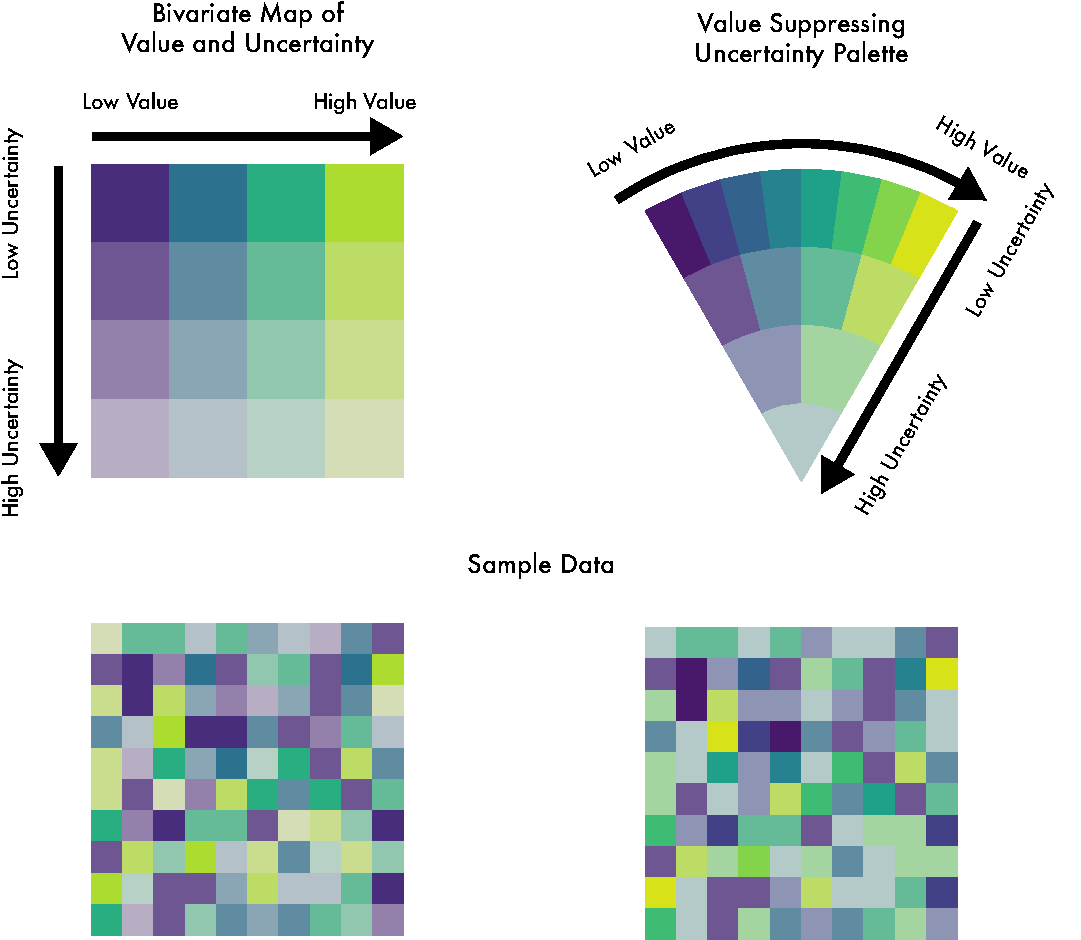
\includegraphics[width=0.9\textwidth]{example.pdf}
		\caption{Lookit! Lookit!}
		\label{fig:teaser}
	}
}

\newcommand{\exampleFig}{
\begin{figure}
	\centering
	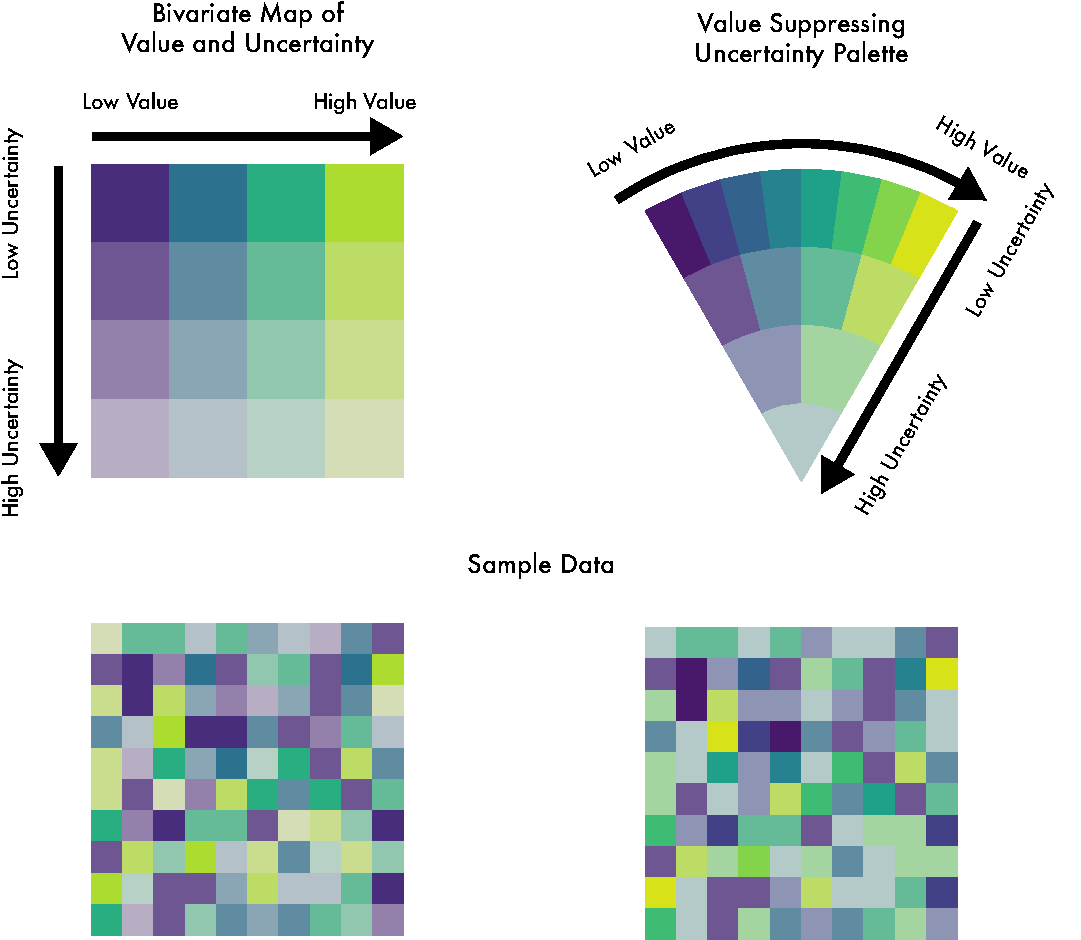
\includegraphics[width=0.9\columnwidth]{example.pdf}
	\caption{A comparison between a standard bivariate map and a VSUM. Both use the same visual channels to encode value (position along the Viridis color map) and uncertainty (lightness and saturation), and have an equal standard of perceptual discriminability (at least 18 units of distance in CIELAB color space between colors). However, highly uncertain values result in colors that are very close together in the bivariate case, meaning the full bivariate map is only 9 bins under these constraints--- a 4x4 map would result in colors that are perceptually too close together. By contrast, the VSUM intentionally reduces bins when uncertainty is high, eventually aliasing all highly uncertain values to the same color. This decision affords more distinct colors in other regions of the map, and so an increase in overall bins to 15. The resulting map suppresses the value of uncertain data, but increases the discriminability of highly certain data.}
	\label{fig:example}
\end{figure}

}

%\teaserFig
%% A teaser figure can be included as follows, but is not recommended since
%% the space is now taken up by a full width abstract.
%\teaser{
%  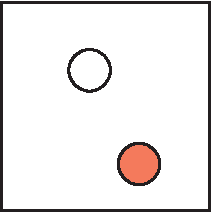
\includegraphics[width=1.5in]{sample.eps}
%  \caption{Lookit! Lookit!}
%}

%% Abstract section.
\abstract{

	% uncertainty-aware decisions.
	% refrain from making a decision
	% integrate uncertainty with the display
	% value-suppressing encodings
	% provide greater visual discriminability for values with high certainty, but alias together uncertain values
	% ran a study
	% results indicate X

Uncertainty is a vital concern in many datasets. Visualizations often use bivariate mappings to encode value and uncertainty simultaneously. Due to interference between visual channels, these bivariate maps are limited in discriminability. We contribute Value-Suppressing Uncertainty Maps (VSUMs), an encoding technique that intentionally impairs value discrimination as uncertainty increases. In contrast to traditional bivariate maps, VSUMs alias values when uncertainty is high: expected values with lower uncertainty can be more precisely compared, whereas similar values with higher uncertainty are made harder to differentiate. By making informed binning decisions, VSUMs seek to better use the limited budget of discriminable marks in bivariate maps, and dissuade analysts from making decisions based on data with high uncertainty. We demonstrate several examples of VSUMs and present a crowdsourced evaluation showing that, compared to traditional bivariate maps, VSUMs bias analysts to more heavily weight uncertainty information in decision-making tasks.

} % end of abstract

%% ACM Computing Classification System (CCS).
%% See <http://www.acm.org/class/1998/> for details.
%% The ``\CCScat'' command takes four arguments.

\keywords{Uncertainty Visualization, Color Perception, Thematic Maps, Semiotics.}

%\CCScatlist{
%  \CCScat{K.6.1}{Management of Computing and Information Systems}%
%{Project and People Management}{Life Cycle};
%  \CCScat{K.7.m}{The Computing Profession}{Miscellaneous}{Ethics}
%}

%% Copyright space is enabled by default as required by guidelines.
%% It is disabled by the 'review' option or via the following command:
% \nocopyrightspace

%%%%%%%%%%%%%%%%%%%%%%%%%%%%%%%%%%%%%%%%%%%%%%%%%%%%%%%%%%%%%%%%
%%%%%%%%%%%%%%%%%%%%%% START OF THE PAPER %%%%%%%%%%%%%%%%%%%%%%
%%%%%%%%%%%%%%%%%%%%%%%%%%%%%%%%%%%%%%%%%%%%%%%%%%%%%%%%%%%%%%%%%

\begin{document}

%% The ``\maketitle'' command must be the first command after the
%% ``\begin{document}'' command. It prepares and prints the title block.

%% the only exception to this rule is the \firstsection command
\firstsection{Introduction}

\maketitle

%% \section{Introduction} %for journal use above \firstsection{..} instead


% What this section needs to do:
% Uncertainty is important!
% What do we mean by ``well-integrated'' uncertainty?
% Scope down to thematic maps
% Juxtapose/superimpost distinction?
% Position bivariate maps (tacitly or explicitly) as state of the art
% Teaser image showing what we mean

Uncertainty is an inescapable component of collecting, presenting, and using data. A common goal in the communication of uncertainty is promoting \emph{uncertainty-aware decisions}: the audience should be aware of the risks and rewards of certain decisions, modulate their confidence in their conclusions, and perhaps refrain from making a decision at all if there is too much uncertainty.  A way that designers can contribute to this goal is by ensuring that uncertainty information is \emph{well-integrated} with the rest of the data. That is, it should be difficult to discount or ignore the uncertainty in a dataset.

Simultaneous presentation of uncertainty and value necessitates the construction of a bivariate map\,---\,a relation, in terms of visual variables, between 2-tuples $(\text{value}, \text{uncertainty})$ and mark properties. The design of bivariate maps is difficult and, due to the interference and interplay between different visual variables, often leads to maps with few discriminable categories.

In this paper, we contribute \textbf{Value-Suppressing Uncertainty Maps} (VSUMs) for integrating data and uncertainty information in thematic maps. VSUMs intentionally alias together data values with high uncertainty, affording greater discriminability as uncertainty decreases. Rather than a traditional two-dimensional bivariate map, with differing outputs for each combination of value and uncertainty, VSUMs can be thought of as arcs: as uncertainty increases, values are mapped to smaller and smaller sets of outputs, culminating in a singularity where all inputs are mapped to an identical, highly uncertain mark regardless of their data value. \figref{fig:example} shows examples of both a VSUM and a more traditional bivariate map.

We describe the motivations behind the use of VSUMs, examples of their utility for decision-making under uncertainty, and assess VSUMs in a crowdsourced experiment. Our experimental results indicate that VSUMs promote better integration between uncertainty and data: X.

\exampleFig
\section{Related Work}

% What this section needs to do:
% State of the art in uncertainty vis, with heavy emphasis on MacEachren & co.
% Bivariate maps are hard!
% Binning colormaps is de rigueur
% The variables we'd want to use for uncertainty (like value or alpha or size) mess with color discriminability

Despite the acknowledged importance of uncertainty in understanding data, explicit representations of uncertainty are often missing from visualizations~\cite{boukhelifa2009uncertainty}. This is partially due to the complexity of uncertainty as a concept. In typologies from Thomson et al.~\cite{thomson2005typology} and Buttenfield \& Beard~\cite{buttenfield1994graphical}, the authors note that many, occasionally contradictory, concepts can fall under the category of ``uncertainty,'' including data quality, sampling error, credibility, and provenance.

Reviewing the state of the art in uncertainty visualization in the field, Greithe et al.~\cite{griethe2006visualization} and Brodlie et al.~\cite{brodlie2012review} present lists of potential techniques for conveying uncertainty in concert with data. Some of these options (interaction, animation, and sonification) are not applicable for static charts; even for dynamic charts, many users do not interact with charts in sufficient detail to recover uncertainty information~\cite{nyt2016}. While we acknowledge the potential utility of these techniques in uncertainty visualization (for instance, the animation used to convey sampling error in Hullman et al.'s \emph{HOPs}~\cite{hullman2015hypothetical}), we limit the scope of our discussion to techniques which center on static charts.

To support our goal of making uncertainty information well-integrated with data, we focus on the techniques of \emph{juxtaposition} (where uncertainty is presented alongside the data), \textbf{superposition} (where additional glyphs are overlaid on top of the data), and \emph{explicit encoding} (where an additional visual channel is used to encode the uncertainty). Gleicher et al.~\cite{gleicher2011visual} explore these three strategies from the perspective of affording \emph{comparisons}; here, we examine them from the perspective of uncertainty visualization.

\subsection{Strategies for Encoding Uncertainty}

\emph{Juxtaposition} creates two explicit visualizations: an ``uncertainty map'' and a ``data map.'' MacEachren~\cite{maceachren1992visualizing} portrays uncertainty visualization as the design problem of how to \emph{unify} these two maps, and so this explicit separation can be counterproductive to the goal of information fusion. Juxtaposition also creates an additional search task for viewers, who must register hot spots in one map with corresponding features of the other map. Nevertheless, especially in cases where the quantification of uncertainty is a separate analysis process from the measuring of data values, juxtaposition is a common design tactic for conveying uncertainty.

\emph{Superposition}, or the overlay of glyphs representing uncertainty on top of a data map, is another common strategy. Error bars are a common example of this strategy: a mark indicating measurement error is superimposed atop a mark representing a point value. Ware's~\cite{ware2009quantitative} \emph{textons} are an example of this strategy applied to thematic maps: monochrome glyphs that can encode an ordinal variable, or a binned quantitative variable. Greithe et al.~\cite{griethe2006visualization} and MacEachren~\cite{maceachren1992visualizing,maceachren1998visualizing} present other examples of superimposed uncertainty in thematic maps, including overlaid grids with ``fuzzy'' lines to indicate uncertainty, or overlaid treemaps with coarser and coarser resolution in uncertain regions. Costs to this approach include obscuring the underlying data map (which can cause uncertainty information to dominate the display~\cite{brodlie2012review}), potential visual interactions that can impair the legibility of glyphs (for instance, simultaneous contrast effects), and the necessity of performing spatial binning in order to ensure that there are a discrete number of uncertainty glyphs. How this binning is performed can introduce undesirable artifacts on the resulting visualization, suppressing important signals or highlighting spurious ones~\cite{battersby2016shapes}.

\emph{Explicit encoding} directly represents uncertainty with a visual channel, simultaneously with data. VSUMs employ this strategy. In addition to overcoming the drawbacks of the other techniques mentioned in this section, we believe that explicit encoding represents the most general form of the solution of how to fuse uncertainty information with data. The most pressing design decisions for explicit encoding are 1) which visual variable to use to encode uncertainty and 2) how to design bivariate maps which afford the encoding of both value and uncertainty. We deal with these two questions in greater detail below.

\subsection{Visual Variables for Representing Uncertainty}

The decision to explicitly encode uncertainty increases the dimensionality of the data, and so requires the use of (at least one) additional visual channel ~\cite{brodlie2012review}. Uncertainty therefore inherently increases the visual complexity of a visualization. When the data are already complex to convey, and many of the more common or accurate visual variables are in use, allocating an additional dimension is non-trivial. As the number of dimensions increases, finding visual variables that are both perceptually accurate (in either estimation of quantity or discrimination of category) as well as perceptually separable from all the other encoding channels, becomes more and more difficult.

A further hurdle is that not all visual variables are well-suited for conveying uncertainty. MacEachren et al.~\cite{maceachren2012visual} evaluate a number of visual variables with respect to their \emph{semiotic fit} for representing uncertainty. They observe that certain visual variables such as blurriness and transparency seem to have a more intuitive connection to uncertainty than other variables such as shape or hue. Unfortunately, Boukhelifa et al.~\cite{boukhelifa2012evaluating} find that many visual variables habitually used for conveying uncertainty, such as blur and value, are also difficult to estimate. This results in a preference/performance gap where designers must choose between encoding uncertainty in a way that is intuitive but error prone, or use higher fidelity channels that may be more difficult to interpret.

\subsection{Bivariate Maps}

For visualizations such as choropleth maps, heatmaps, or treemaps, visual channels such as position and length are reserved for data variables other than value (such as geographic location or relative size). In these situations, data value is often encoded using color. Colors in such univariate quantitative color maps should be sufficiently far apart as to be perceptually distinguishable~\cite{ware1988color}, and vary in lightness as well as hue in order to afford an implicit ordering of value~\cite{borland2007rainbow,rogowitz2001blair}. Different choices of color maps can highlight different features of the data, and should be chosen with care based on the data types and important features to be visualized~\cite{rogowitz1996not}.

Given these considerations, and the perceptual integrality of color channels, the construction of \emph{bivariate} color maps is difficult. Viewers need to be able to independently assess the variables of interest, but the resulting bivariate map should also be expressive and easy to interpret. Bivariate maps with these constraints are often limited to relatively few categories (say, a 3x3 matrix as in \figref{fig:example}) \cite{robertson1986generation,trumbo1981theory}. In general, the quality of bivariate color maps is a multivariate measure involving consideration of not just the component color channels, but also the interpolation scheme and the color of the surround~\cite{bernard2015survey}. However, even simple bivariate maps can be difficult for a general audience to interpret \cite{wainer1980empirical}.

Dunn~\cite{dunn1989dynamic} attempts to circumvent these issues by dynamically allocating bins to the bivariate map. As the number of distinct, separable colors is limited, the dynamic approach allocates bins to regions of the highest utility. For instance, placing the dividing line between bins in areas aligned with a trend line allows the color to encode information about the sign of the residual with respect to each variable. This insight, that the bins in a bivariate map are a limited resource and so should be ``spent'' wisely, drives the creation of VSUMs, which allocate more bins in a bivariate map to regions with less uncertainty.

\section{Value-Suppressing Uncertainty Maps}

Value-Suppressing Uncertainty Maps (VSUMs) are a technique for creating bivariate maps of data \emph{value} and \emph{uncertainty}. These maps circumvent the issues in the creation of traditional bivariate maps by making the following assumptions:

\begin{enumerate}
	\item \textbf{Designers have a limited budget of discriminable marks.} That is, viewers cannot easily or reliably discriminate between an infinite number of categories. Rather than accept this perceptual ambiguity, designers ought to \emph{alias} together marks into a finite, but sufficiently discriminable, set.
	\item \textbf{Uncertain values should have less weight than certain values.} Weight, in this case, might mean literal visual weight, or impact on the decision-making process.
\end{enumerate}

%MC this paragraph is a little iffy, and sort of "the lady doth protest too much" territory. we might be able to get away with "people bin colors all the time. and in fact, you really should be binning your colors anyway."
The first assumption seems to contradict Mackinlay's \emph{expressiveness principle}~\cite{mackinlay1986automating}, where the visual encoding of the data should reflect the composition of the data. For instance, if my data are a collection of measurements of some continuous variable, then it would make sense to encode these data using a continuous \emph{visual} variable, which would then mean an arbitrary number of potential marks. For instance, a bar can have an arbitrary, non-integer height. However, for many visualizations, the perceptual ambiguity caused by having marks that cannot be reliably disambiguated is higher than the gain from having a visual encoding that maps readily to the backing data. Padilla et al.~\cite{padilla2017evaluating} present one such example, where binned heatmaps result in higher task accuracy than continuous heatmaps.

In some cases, this second assumption is violated. For instance, an analyst might be interested in ``long tail risks'' or other ``black swan events,'' where the impact of an value, no matter how uncertain, must be considered and planned for~\cite{taleb2011black}. Other analysis tasks (such as filtering out outliers), require increased, rather than decreased, discriminability when uncertainty is high. However, for many information fusion tasks, the assumption is that uncertainty is related to data quality, or the uncertainty of particular data values~\cite{riveiro2007evaluation}. As with null hypothesis significance testing, the aim would then be to avoid Type I errors, where patterns arising from statistical noise or measurement error are interpreted as significant signals.

If both of these assumptions hold, then it follows that the designer of a bivariate map should allocate more mark types to certain values, and fewer mark types to uncertain values. VSUMs codify this decision by \emph{reducing the number of mark categories for representing value as uncertainty increases.} This means that data encoded using a VSUM will make visible only the largest of differences in uncertain data, but highlight comparatively small differences in value when uncertainty is low. VSUMs therefore act as both a filtering mechanism (in that values with too much uncertainty are all mapped to the same glyph), as well as an implicit test of effect size (in that smaller and smaller changes in value are visible as uncertainty decreases). This strategy of dampening the low quality or high uncertainty values in maps in order to focus on more informative regions has measurable benefits, including the removal of statistically spurious visual patterns, and the highlighting of regions of interest~\cite{correll2017surprise}.

\subsection{Method}

The general VSUM algorithm is as follows:

\begin{enumerate}
	\item \textbf{Select a visual variable to encode value}. In most cases in this paper, this variable is position along some established color scale.
	\item \textbf{Select a visual variable to encode uncertainty}. We prefer variables that have a somewhat high semiotic connection with uncertainty (such as lightness and size), but still have a reasonable number of perceptually discriminable layers (as opposed to other, more intuitive channels such as blur or sketchiness).
	\item \textbf{Select a discriminability threshold}. Choose some minimum distance, in a perceptual space, between marks. For many visual variables (such as length or hue), the perceptual discriminability between marks has been assessed in prior literature, and so the only step is to choose a value in terms of the just noticeable distance (JND). For less common visual variables, a perceptual model may be built empirically (as in Demiralp et al.~\cite{demiralp2014learning}).
	\item \textbf{Choose how quickly categories \emph{degrade}}. That is, if there are $n$ bins at some uncertainty level $m$, how many bins should there be when uncertainty increases to level $m+1$? In \figref{fig:example}, this function is $\left \lfloor {\frac{n}{2}}\right \rfloor$, meaning that the number of value bins decreases by half for each level of uncertainty bins. If there is too much degradation, then there are fewer levels of uncertainty. If there is no degradation, the resulting map is just a traditional bivariate map.
	\item \textbf{Choose the largest number of initial categories $n$ such that the discriminability threshold is met.} For each pair of marks in the map, perform a pairwise comparison of discriminability. If no marks are perceptually ambiguous by the standards of your threshold, the map is complete. Otherwise, decrement $n$.
\end{enumerate}

Figure X shows this process in detail, and how it can be used to generate a bivariate map for presenting uncertainty. JavaScript code for generating VSUMs given arbitrary d3 quantitative scale functions is available at \url{URL REMOVED FOR REVIEW}.

Correll et al.~\cite{correll2015layercake,correll2011visualizing} use a pre-cursor of VSUMs in their LayerCake genomics visualization tool, where marks representing genomic data with increasing uncertainty are mapped to a smaller and smaller set of increasingly grey colors, creating the effect of uncertain values retreating into ``fog'' while highly certain values remain prominent. Other bivariate visualizations implicitly alias together uncertain values. For instance, if uncertainty is encoded by transparency, a maximally uncertain glyph may be entirely transparent, and so impossible to distinguish from any other maximally uncertain glyph. Other channels with a semiotic connection to uncertainty, such as saturation, value, blur, or size, also have deleterious effects on the disambiguation of colors and shapes. In both of these cases, the property of aliasing is \emph{ad hoc}, and places no guarantees on the discriminability of colors. The binning and degradation approach of VSUMs makes the choice to alias values explicit to both the designer and the viewer, and results in a bivariate mapping with known perceptual properties.

\subsection{Design Considerations}

\performanceFig

There are multiple choices that designers must make before creating a VSUM. In particular, they must choose 1) which visual channels map to value and uncertainty, 2) a threshold of perceptual distinguishability (and, implicitly, a corresponding metric), and 3) a degradation function to determine how quickly uncertain values are aliased.

Often, the graphical conventions of a chart reserve variables such as position and area for other uses, and determine the visual channel to be used for value. In thematic maps, for instance, value is regularly encoded using color, while vertical and horizontal position are reserved for location. In this paper, we primarily deal with the case where value is encoded using color. While there are some similar conventions for representing uncertainty, generally designers have a greater degree of freedom in choosing a visual channel for uncertainty~\cite{maceachren1992visualizing}. We recommend channels with both a strong semiotic connection to uncertainty as well as a relatively large number of perceptually distinguishable levels. Here, we focus on value/saturation (or, equivalently, transparency against a white background) and size. Correll \& Gleicher~\cite{correll2013error} show that even audiences without statistical backgrounds can interpret uncertainty information encoded in these channels.

Another reason for limiting our discussion of bivariate mappings to color and size channels is that the perceptual distinguishability of these channels has been well-studied by prior work. CIELAB and other color spaces are designed to approximate perceptual uniformity\,---\,that is, distance in the color space should universally correspond with perceptual distance. Recent work~\cite{stone2014engineering,szafir2014adapting} has investigated the discriminability of colors in such spaces not only under laboratory conditions, but also among the disparate display conditions and color vision proficiency of crowdworkers. Similarly, formative work by Cleveland \& McGill~\cite{cleveland1984graphical} assesses the discriminability of marks of different height, and this too has been extended both to a larger population of crowdworkers, and to the area channel specifically~\cite{heer2010crowdsourcing,talbot2014four}.

We use values from these works as benchmarks for selecting thresholds of discriminability. The ``just noticeable difference'' (JND) of these channels provides a useful minimum; in practice, we would wish to create maps with marks that are far more reliably distinguishable than the 50\% or 75\% discriminability rate of a JND. \figref{fig:performance} shows how these benchmarks can be used to select reasonable thresholds. Other factors, such as nameability and aesthetic preference, can be added in as additional weights impacting the desirability of certain color palettes, as in Gramazio et al.~\cite{gramazio2017colorgorical}.

How quickly the number of bins decreases is another parameter of VSUMs. If this degradation is too large, then we may only have a few discriminable levels of uncertainty. If this degradation is too small, then we can be overwhelmed with colors. For instance, if we only decrement by one bin per level of uncertainty, there would be \emph{1,485} different colors in a VSUM with a tolerance threshold of $1$ unit in CIELAB space. In the examples in this paper,  we halve the number of bins at each increasing level of uncertainty. When the initial bins at the highly certain region is a power of $2$ (as in Fig. \ref{fig:example}), this imparts a tree structure to the resulting VSUM. As uncertainty increases, bins in the previous level map to one and only one ``parent'' in the next uncertainty level, resulting in fewer crossings of color boundaries among rows.

\subsection{Examples}

Every pair of colors quantized color maps should be easily distinguishable from any other color in the color map. VSUMs have a lower resolution for uncertain values and thus can have higher resolution for values with high certainty. We created 2D uncertainty maps and VSUMs and used them to visualize flight delay data and mutations in viral genomes to show that VSUMs have higher discriminability where it matters.

The airline delay visualization shows average delays for different times of the day and days of the week. In this example we used data about flight delays of US carriers from the Bureau of Transportation Statistics~\cite{bts} for January 2017. In addition to the average delay for each pair of time of the day and day of the week, we computed the standard error of the mean as the standard deviation divided by the squareroot of the number of samples.

\airlineFig

\figref{fig:airline2d} shows the heatmap visualization where the delay and uncertainty are encoded with a 2D uncertainty map. We used a minimum discriminability  threshold of $18$ units in CIELAB space. We can see that the lowest delays are early in the day throughout the week. With the same threshold we can create a VSUM with much higher resolution for values with high certainty (\figref{fig:airlineVsum}). The VSUM also has more resolution for the uncertainty (4 different levels instead of 3 in the 2D heatmap). If the analysts is interested in delay patterns, VSUMs give them higher resolution. Since VSUMs blend uncertain values together, 2D maps are better if analysts are interested in high expected delays independent of the uncertainty. However, if analysts want to investigate uncertainty or values in isolation, separate channels (\eg juxtaposed heatmaps) are better as they prevent interaction effects. 

\viralFig

In \figref{fig:viral2d} and \figref{fig:viralVsum}, we visualized the mutation rate of virus genomes. Biologists know that certain regions of the genome are ``coding regions'' that influence the the formation of proteins. The data you see here, however, has errors because the process of reading the genome is not perfect. Similarly to the flight delay example, the resolution for certain values with 2D uncertainty maps is much lower (\figref{fig:viral2d}). VSUMs enable biologists to see more fine grained differences as shown in \figref{fig:viralVsum}.


\section{Evaluation}

\conditionFig

We performed a crowdsourced experiment on Amazon's Mechanical Turk in order to evaluate the effectiveness of VSUMs for integrating uncertainty and value information in thematic maps. This focus on integration meant that we limited our experimental tasks to scenarios where the participants needed to consider both value and uncertainty before making a decision. We gave participants two main tasks:

\begin{enumerate}
	\item [T1] an \textbf{identification} task, where we gaves participants charts with value and uncertainty information, and asked them to locate specific regions. E.g., ``click on the region of the chart with highest uncertainty \emph{and} lowest value.''
	\item [T2] a \textbf{prediction} task, similar to Battleship, where we gave participants charts with both \emph{forecast} and \emph{forecast uncertainty} information, and asked the participants to place tokens on the board in order to optimize expected value. E.g., ``place your $4$ ships on safe locations on the board.''
\end{enumerate}

We discuss the two experimental tasks in more detail in the following sections.

For each task, participants saw one of three types of thematic maps. Either two \textbf{juxtaposed} maps side-by-side, with separate encodings for value and uncertainty, a traditional \textbf{bivariate} map, where value and uncertainty are orthogonally encoded, or a \textbf{VSUM}. Figure \ref{fig:stimuli} shows examples of these factor levels. Other factors included the size of the map (either a 4x4 or 8x8 grid), and (for the prediction task), the question framing (attack or defense). These secondary factors were evenly blocked across stimuli. Fatigue effects were significant in piloting, and so we limited the number of replicates: participants saw 18 stimuli (6 for each map type) for the identification task, and 12 (4 for each map type) for the prediction task. 

In all cases, we generated color maps based on the requirement that no two colors in the resulting color scheme were closer than 18 units of Eulcidean distance in CIELAB space. This threshold results in a $9$ color bivariate map, $15$ color VSUM for all color scales used in this study. Given the size of the marks used in our study, this threshold distance is sufficient for colors to be correctly distinguished in over 95\% of trials~\cite{stone2014engineering}. Other choices of threshold, and differing univariate scales, would result in different maps (see Fig.~\ref{fig:performance}). 


\subsubsection{Identification Task}

For the identification task, we gave participants bivariate representations of uncertainty, and asked them in a written prompt to identify a location meeting a given criteria, e.g., ``Click on the location with the greatest uncertainty.'' There were three potential criteria, mapping to the three vertices of a VSUM: 1) high value, low uncertainty, 2) low value, low uncertainty, and 3) high uncertainty. Each map contained four locations, one of each combination of maximum and minimum value and uncertainty. The correct answer was always one of these locations. Other locations in the grid were created pseudo-randomly, with less extreme ranges of uncertainty and probability. We measured performance both in terms of accuracy (did the participant select the correct point) as well as response time.

\subsubsection{Prediction Task}

\taskTwoFig

For the prediction task, we gave participants the rules of a game similar to Battleship. Greis et al.~\cite{greis2016decision} employ these game-like experimental tasks to frame uncertainty information, which can be abstract or complex, to the general audience. In our task, the participant and a (fictional) adversary have to place tokens representing ships on a spatial grid. Without direct access to the location of the opponent's ships, the player then has to place tokens representing missile strikes on their opponent's grid. Players had to place all of their tokens before continuing. If a player fires a missile at a square containing a ship, then that ship is sunk. The objective is the maximize the number of enemy ships hit, while minimizing the number of your own ships that are hit. In our task, participants were given a chart encoding predictions on the location of enemy ships (in the attacking case) or potential missile strikes (in the defending case). The \emph{value} component of the prediction was the likelihood of a item being present in a particular region. The \emph{uncertainty} component was the confidence in this prediction.

We included both a \textbf{gain} framing (given predictions of where your opponent's ships are, where should you launch your missiles?), and a \textbf{loss} framing (given predictions of where your opponent's missiles will fall, where should you place your ships?) in order to account for systematic differences in human judgments under uncertainty. Tversky \& Kahneman~\cite{tversky1985framing} illustrate that framings in terms of gains or losses produce reliably different outcomes. In general, the function of the value of gains is concave, but is convex for losses~\cite{kahneman1979prospect}. That is, avoiding a large loss is often more valuable than striving for a similarly large gain. To avoid potential (in this case, incorrect) transfer learning, the attacking and defending used different value color maps (Plasma and Cool) than the identification tasks, and from each other.  Figure \ref{fig:taskTwoConditions} shows these differing color maps and framings.

The ideal strategy from a value-maximizing standpoint would be to place tokens on areas with the highest expected value, ignoring the uncertainty information. However, as with Roulette and other similar games of chance, the variability in expected value is relevant when considering where to place bets~\cite{mlodinow2009drunkard}. Over the short term, a player may seek out high expected value but risky locations, or, if risk averse, accept lower expected value but lower variability locations. We therefore measured the distribution of both \emph{value} and \emph{uncertainty} of the tokens placed by the participants. Each map contained a minimum number of ``risky'' locations: cells with high expected value, but also high uncertainty. There were also an equal number of ``safer'' locations, with slightly less expected value, but also less uncertainty. The remaining locations of the map varied pseudo-randomly in the middle ranges.

%Show:
% 1) Juxtaposition makes people ignore/underweight uncertainty (even when they don't screw up the search task)
% 2) VSUMs make people, surprise surprise, bad at distinguishing highly uncertain values
% 3) But, they make uncertainty better-integrated
%    i) lower weights on uncertain values in decision-making
%    ii) a priori better discrimination

%conditions:
% 1) juxtaposed d map, u map
% 2) binned d/u map as per a priori jnds
% 3) vsm
% 4) continuous d/u map?

\subsubsection{Hypotheses}

We had several hypotheses, stemming from our believe that VSUMs promote better \emph{integration} between uncertainty and value information, and also encourage \emph{caution} by highlighting the ambiguity or untrustworthiness introduced by uncertain data. In particular:
\begin{enumerate}
	\item Participants would be \textbf{faster and more accurate} when completing the identification task using a VSUM as compared to the other map types. Juxtaposed maps, by adding an additional search task to the lookup task, would have especially poor performance compared to VSUMs.
	\item Participants would choose targets with \textbf{less uncertainty} in the prediction task when using a VSUM compared to the other maps types. This would result in a tradeoff where they would also choose targets with \textbf{less expected value} than the other map types. Again, juxtaposed maps, by increasing the difficulty of retrieving both variables simultaneously, would highlight this difference.
\end{enumerate}

\subsection{Results}

\subsubsection{Participants}

We limited our population to Turkers from the United States, with a prior task approval rate of at least 90\%. As the experimental tasks required multi-hue color perception, we presented participants with a set of Ishihara plates as a pretest, and excluded participants who either misidentified the values in the plates, or who self-reported as having a color vision deficiency (CVD) in the post-test. Based on piloting, we paid participants \$2 dollars an hour, for a target rate of \$8/hour. After completion of the main tasks, we solicited demographic information, and performed a domain-agnostic general risk aversion assay~\cite{mandrik2005exploring}.

\section{Discussion}
\subsection{Limitations and Future Work}
% When should you use these things?

\section{Conclusion}


%% if specified like this the section will be committed in review mode
\acknowledgments{
Omitted for review.}

%\bibliographystyle{abbrv}
\bibliographystyle{abbrv-doi}
%\bibliographystyle{abbrv-doi-narrow}
%\bibliographystyle{abbrv-doi-hyperref}
%\bibliographystyle{abbrv-doi-hyperref-narrow}

\bibliography{template}
\end{document}
